\documentclass[../main.tex]{subfiles}
\graphicspath{{figures/}{../figures/}}
\usepackage{graphicx}
\begin{document}
% \todo[color=green!30]{完成问题一模型的建立(sections/q1\_build)}

\noindent \textbf{5.1.1.1回焊炉内的温度分布模型的确立}

\par 以炉前区域左边边缘为原点,向右建立一维坐标轴,简化回焊炉模型。
\par 根据题目可知,回焊炉启动后,炉内空气温度会在短时间内达到稳定性,炉内各点温度处于稳态。并且,回焊炉的加热主要依靠外部加热系统,内部没有持续且显著的热源产生热量影响温度分布,因此,回焊炉无内热源。以及根据题意可知,回焊炉内满足常物性。从而我们可以得到拉普拉斯(Laplace)方程:
\begin{align}\label{1.1}
    \frac{\mathrm{d}^2T}{\mathrm{d}x^2}=0
\end{align}
\par 其中,$x$表示坐标轴上的点与原点之间的距离,$T$表示在回焊炉内$x$点处的空气温度。对\eqref{1.1}两次积分求解可得下列式子,$C_1$,$C_2$为任意常数。
\begin{align}\label{1.2}
    T\left( x \right) =C_1x+C_2 
\end{align}
\par 由于炉内空气温度达到稳定后,各小温区温度达到恒定,为其设定温度。并且,炉前区域,炉后区域以及小温区之间的间隙温度与相邻温区的温度有关,因此可以据题目给定的已知条件求得回焊炉内的温度$T$沿空间位置$x$的分布关系
\par \textbf{step 1 炉前区域的温度分布}
\par 在一维坐标轴上,炉前区域表示为$x\in \left[ 0,25 \right] $,据题意可知,生产车间温度 \(T_0\) 为 \(25^{\circ}C\),小温区 \(1\sim5\) 的温度 \(T_1\) 为 \(175^{\circ}C\)。
因此,存在点 \(a\) 使得:
\begin{align}
T(0\leq x\leq a)& = 25^{\circ}C \label{1.3}\\
T(a < x < 25)&> 25^{\circ}C  \label{1.4}
\end{align}
\par 又因为,从 \(a\) 点处开始的温度变化为线性变化,且 \(T(x = 25)=25^{\circ}C\),结合 \(T_0\),\(T_1\) 以及从 \(a\) 点处开始的温度变化区间和 \eqref{1.2} 式,可得炉前区域的温度分布:
\begin{gather}\label{1.5}
T(x)=\begin{cases}
25 & (0\leq x\leq a) \\
25+\frac{150}{25 - a}(x - a)&(a \leq x \leq 25)
\end{cases}
\end{gather}
\par \textbf{step 2 炉内区域的温度分布}
\par 在一维坐标轴上,小温区$1\sim 5$(包含间隙$1 \sim4$ ),表示为 \(x\in[65,197.5]\) ,因为小温区$1\sim5$的温度 \(T_{1}\) 为 \(175^{\circ}C\) ,据\eqref{1.2}式可得,间隙$1\sim4$的温度均为 \(175^{\circ}C\) ,因此
\begin{align}\label{1.6}
T(x)=173\quad(25\leq x\leq197.5)
\end{align}
\par 在一维坐标轴上,小温区6表示为 \(x\in[202.5,233]\) ,由题意可知,小温区6的温度 \(T_{2}\) 为 \(195^{\circ}C\) ,因此
\begin{align}\label{1.7}
  T(x)=195\quad(202.5\leq x\leq233)
    \end{align}
    \par 在一维坐标轴上,小温区7表示为 \(x\in[238,268.5]\) ,由题意可知,小温区7的温度 \(T_{3}\) 为 \(235^{\circ}C\) ,因此
\begin{align}\label{1.8}
  T(x)=235\quad(238\leq x\leq268.5)
    \end{align}
\par 在一维坐标轴上,小温区$8\sim9$(包含间隙8 ),表示为 \(x\in[273.5,339.5]\) ,因为小温区$8\sim9$的温度 \(T_{4}\) 为 \(255^{\circ}C\) ,据\eqref{1.2}式可得,间隙8的温度为 \(255^{\circ}C\) ,因此
\begin{align}\label{1.9}
T(x)=255\quad(273.5\leq x\leq339.5)
    \end{align}
\par 在一维坐标轴上,小温区$10\sim11$(包含间隙10 ),表示为 \(x\in[344.5,410.5]\) ,因为小温区10 - 11的温度 \(T_{5}\) 为 \(25^{\circ}C\) ,据\eqref{1.2}式可得,间隙10的温度为 \(25^{\circ}C\) ,因此
\begin{align}\label{1.10}
    T(x)=25\quad(344.5\leq x\leq410.5)
    \end{align}
\par 在一维坐标轴上, 间隙5表示为 \(x\in[197.5,202.5]\) ,因为相邻两个区间温度分别为 \(T_1\),\(T_2\),因此据\eqref{1.2}式可得:
\begin{align}\label{1.11}
   T(x)=175 + 4x\quad(197.5\leq x\leq202.5)
    \end{align}
    \par 在一维坐标轴上, 间隙6表示为 \(x\in[233,238]\) ,因为相邻两个区间温度分别为 \(T_2\),\(T_3\),因此据\eqref{1.2}式可得:
    \begin{align}\label{1.12}
       T(x)=195 + 4x\quad(233\leq x\leq238)
        \end{align}
\par 在一维坐标轴上, 间隙7表示为 \(x\in[268.5,273.5]\) ,因为相邻两个区间温度分别为 \(T_3\),\(T_4\),因此据\eqref{1.2}式可得:
        \begin{align}\label{1.13}
           T(x)=235 + 4x\quad(268.5\leq x\leq273.5)
            \end{align}
            \par 在一维坐标轴上, 间隙9表示为 \(x\in[339.5,344.5]\) ,因为相邻两个区间温度分别为 \(T_4\),\(T_5\),因此据\eqref{1.2}式可得:
            \begin{align}\label{1.14}
               T(x)=255 - 46x\quad(339.5\leq x\leq344.5)
                \end{align}   
\par \textbf{step 3 炉后区域的温度分布}  
\par 在一维坐标轴上,炉后区域表示为$x\in \left[ 410.5,435.5 \right] $,据题意可知,生产车间温度 \(T_0\) 为 \(25^{\circ}C\),小温区 \(10\sim11\) 的温度 \(T_5\) 为 \(25^{\circ}C\)。
因为炉后区域的温度分布为线性分布,从而:
\begin{align}\label{1.15}
    T(x)=25\quad(410.5\leq x\leq435.5)
    \end{align}
    \par \textbf{step 4 回焊炉的温度分布} 
\par 综上所述,回焊炉的温度分布表如下
\begin{table}[H]\label{1.16}
    \centering
    \caption{回焊炉的温度分布表}
    \renewcommand{\arrayrulewidth}{2.0pt}
    \begin{tabular}{c|c|c} 
    \hline
    x & 温区 & 温度  \\ 
    \hline
   $ \left[ 0,25 \right]$& 炉前区域 & $25(0\leq x\leq a) $  \\ 
    \cline{3-3}
      &      & $25+\frac{150}{25 - a}(x - a)(a \leq x \leq 25)$   \\ 
    \hline
    $\left[ 25,197.5 \right]$& 小温区$1\sim5$(包含间隙$1\sim4 $)  & 175 \\ 
    \hline
    $\left[ 197.5,202.5 \right]   $& 间隙5     & $175 + 4x$     \\ 
    \hline
   $ \left[ 202.5,233\right] $ & 小温区6   &  195    \\ 
    \hline
   $ \left[ 233,238 \right] $  &    间隙6   &   $195 + 4x$     \\ 
    \hline
    $ \left[ 238,268.5\right] $& 小温区7     &  235    \\ 
    \hline
 $ \left[ 268.5,273.5 \right] $    &   间隙9   &   $235 + 4x$     \\ 
    \hline
$ \left[ 273.5,339.5 \right] $ & 小温区$8\sim 9$(包含间隙8 )     &   255   \\ 
    \hline
$ \left[ 339.5,344.5 \right] $&  间隙9    &  $255 - 46x$      \\ 
    \hline
$     \left[ 344.5,410.5 \right]$  & 小温区$10 \sim 11$(包含间隙10 )          & 25     \\ 
    \hline
    $\left[ 410.5,435.5 \right]$        & 炉后区域     &   25   \\
    \hline
    \end{tabular}
    \end{table} 

\par 因此,我们可以得到回焊炉各位置的温度分布即传送带各位置达到稳态时的个温度分布$T_{\infty}(x)$.
由题意可知电路板两侧搭在传送带上匀速穿过炉内,且传送带的过炉速度恒为:
\begin{align}\label{1.17}
v_0=70\ cm/min
\end{align}
\par 故而电路板在一维坐标轴上的位置$x$可以用$v_0t$表示,所以上式可化为:
\begin{align}
T_{\infty}(x)=T_{\infty}(v_0t)
\end{align}
\noindent \textbf{5.1.1.2焊接区域的温度分布模型的确立}
\par 通过题目给定条件,我们可以知道焊接区域的厚度$2\delta$为$0.15mm$.由于电路板的材质一般为金属,金属板与空气的传热(对流)系数$h$一般在$5\sim 500\mathrm{W}/(\mathrm{m}^2\cdot\mathrm{K})$内,金属的导热系数$\lambda$一般在$100\mathrm{W}/(\mathrm{m}^2\cdot\mathrm{K})$左右,而厚度$2\delta$很小,所以电路板内部的热阻与外部热阻之比$Bi=\frac{\delta h}{\lambda}\ll 0.1$,因此我们可以用集中参数法,即将整块电路板的内部温度分布近似看作均匀分布来求解此题。
\par 因为题目只给了焊接区域厚度$2\delta$,所以我们忽略水平方向的热对流,只考虑垂直于电路板方向的热对流对电路板温度的影响。
%\par \textbf{step 1 建立竖直方向的热传递方程} 
\par 以焊接区域中心为原点$O$,向上为正方向建立一维坐标轴,如下图所示
\begin{figure}[H]\label{1.18}
\centering
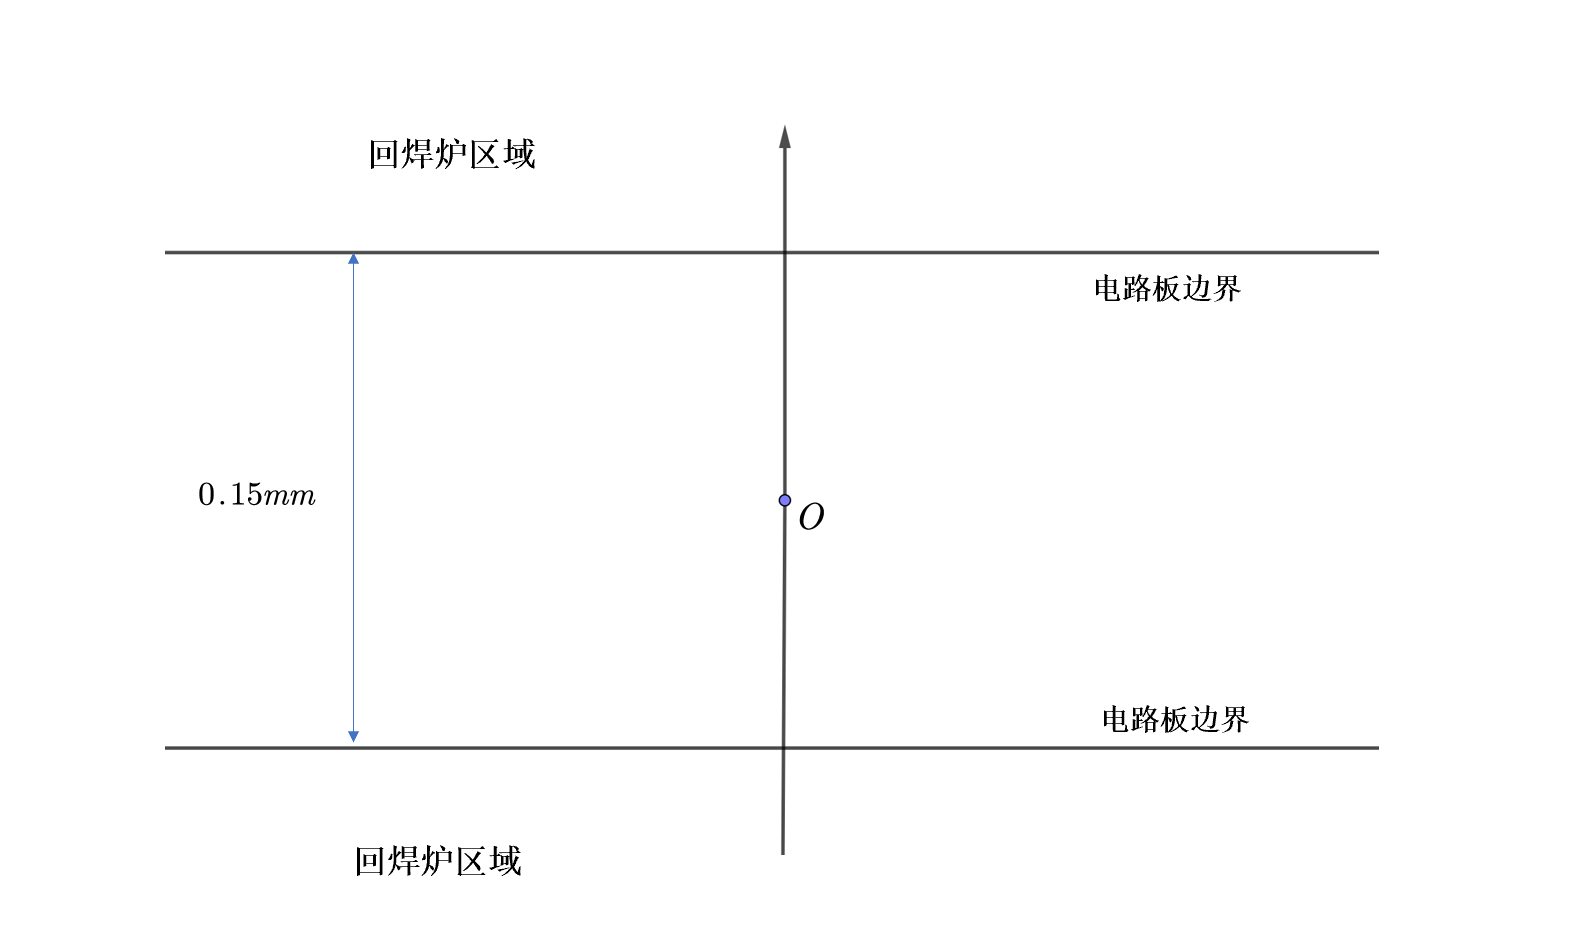
\includegraphics[width=1\textwidth]{7.png}
\caption{焊接区域坐标轴}
\end{figure}\label{1.20}
\par 一维坐标轴上的位置用$y$来表示,因为焊接区域关于焊接中心对称,所以我们只需要考虑电路板上半部分的热对流,即
\begin{align}\label{1.21}
    0\le y\le \delta =0.075mm  
    \end{align}
    \par 据题意可知,焊接区域的温度分布与其在横轴和竖轴的位置有关,横轴的位置$x$可用$v_0t$表示。因此,焊接区域的温度分布与竖轴位置$y$和时间$t$有关。根据热传导方程,我们可以知道焊接区域的温度分布函数$T\left( y,t \right) $ 满足
    \begin{align}\label{1.19}
    \frac{\partial T(y,t)}{\partial t}=a\frac{\partial ^2T(y,t)}{\partial y^2}(0<y<\delta,t>0)
    \end{align}
    \par  其中$a$为热扩散率,与导热系数$\lambda$和$\rho c$($\rho$为电路板密度,$c$为比热容)有关,即
    \begin{align}
    a=\frac{\lambda}{\rho c}
    \end{align}
    \par  记$A=\rho c$,则
    \begin{align}\label{2.2}
    a=\frac{\lambda}{A}
    \end{align}
    %\par \textbf{step 2 确定初值条件,对称和对流边界条件} 
    \par  据题意可知,生产车间温度始终保持$25°\text{C}$,因此其初值条件
    \begin{align}\label{2.3}
    T(y,0)=T_0=25^{\circ}\mathrm{C}(0\leqslant y\leqslant \delta)
    \end{align}  
    \par 因为焊接中心上下传热对称,所以其边界条件
    \begin{align}\label{2.4}
    \frac{\partial T(y,t)}{\partial y}\Big|_{y = 0}=0
    \end{align} 
    \par 电路板在过炉过程中,其表面温度$T\left( \delta ,t \right)$不断变化,周围空气温度$T_{\infty}(v_0t)$也因焊接区域的热影响而改变.因此,据牛顿冷却定律,焊接区域表面与空气之间的热流密度$q$满足
    \begin{align}\label{2.5}
    q = h(T(\delta,t) - T_{\infty}(v_0t))
    \end{align}
    \par 将傅里叶定律用热流密度$q$表示,得到焊接区域内部传导到电路板边界的热流密度,即
    \begin{align}\label{2.6}
    q= -\lambda\frac{\partial T(y,t)}{\partial y}\Big|_{y= \delta}    
    \end{align}
    \par 由于内部传导到边界的热量与边界和空气对流换热的热量平衡,即单位时间内通过单位面积的热量相等,因此其热流密度相等,即
    \begin{align}\label{2.7}
    h(T(\delta,t) - T_{\infty}(v_0t)) = -\lambda\frac{\partial T(y,t)}{\partial y}\Big|_{y= \delta}  
    \end{align}
    \par 为了简化方程,我们引入过余变量$\theta(y,t)=T(y,t)-T_{\infty}(v_0t)$,则方程\eqref{1.19}可化为
    \begin{align}\label{2.8}
    \frac{\partial \theta(y,t)}{\partial t}=a\frac{\partial ^2\theta(y,t)}{\partial y^2}(0<y<\delta,t>0)
     \end{align}
    \par 记
    \begin{align}\label{2.9}
    \theta_0(t)=\theta(y,0)=T(y,0)-T_{\infty}(v_0t)=T_0-T_{\infty}(v_0t)
    \end{align}
    \par 根据过余变量和\eqref{2.4}\eqref{2.7},可以得到以下关系式
    \begin{align}
    &\frac{\partial \theta(y,t)}{\partial y}\Big|_{y = 0}=0     \label{2.10}\\
    &h\theta(\delta,t)=-\lambda\frac{\partial \theta(y,t)}{\partial y}\Big|_{y = \delta}   \label{2.11}
    \end{align}
    \par 联立\eqref{2.3}\eqref{2.8}\eqref{2.10}\eqref{2.11},得到焊接区域温度分布模型为以下方程组
    \begin{align}\label{2.12}
    \left\{\begin{array}{l}
    h\theta \left( \delta ,t \right) =-\lambda \left. \frac{\partial \theta \left( y,t \right)}{\partial y} \right|_{y=\delta}\\
    \left. \frac{\partial \theta \left( y,t \right)}{\partial y} \right|_{y=0}=0\\
    T\left( y,0 \right) =25^{\circ}\text{C\,\,}\left( 0\leq y\leq \delta \right)\\
    \frac{\partial \theta \left( y,t \right)}{\partial t}=a\frac{\partial ^2\theta \left( y,t \right)}{\partial y^2}\,\,\left( 0<y<\delta ,t>0 \right)\\
    \end{array} \right. 
    \end{align}
    \par 利用PDE理论可得到解析解
    \begin{align}\label{2.20}
    \frac{\theta(\eta,t)}{\theta_0(t)}=\sum_{n = 1}^{\infty}{C_n\exp(-\mu_{n}^{2}F_O)\cos(\mu_n\eta)}
    \end{align}
    \par 其中
    \begin{align}\label{1.31}
    C_n=\frac{2\sin(\mu_n)}{\mu_n+\cos(\mu_n)\sin(\mu_n)}
    \end{align}
    \par $\eta $表示把厚度方向归一化,即
    \begin{align}\label{1.32}
    \eta =\frac{Y}{\delta}\left( 0\le \eta \le 1\text{,0表示中心,1表示上表面} \right) 
    \end{align}
    \par  $F_O$为傅里叶数,衡量时间对热扩散的影响,即
    \begin{align}\label{1.33}
    F_O=\frac{at}{\delta ^2}
    \end{align}
    \par $\mu_n$为下列方程的根
    \begin{align}\label{1.34}
    \tan(\mu_n)=\frac{Bi}{\mu_n},n = 1,2,\cdots
    \end{align}
    \noindent \textbf{5.1.1.3 参数估计}
    \par 由一维传热模型可知,$a,\lambda,h$为未知参量。因此,我们只需用最小二乘法估计参数$a,\lambda,h$即可
    \begin{align}\label{4.1}
    \left( \widehat{a},\widehat{\lambda },\widehat{h} \right) =\underset{a,\lambda ,h}{\mathrm{arg}\min}\left( T\left( a,\lambda ,h,\delta,t \right) -T\left( \delta,t \right) \right) 
    \end{align}
    \par 假设空气为低速(静止)空气的情况,因为在自然对流的情况下,温差越大,空气的流动就越剧烈,从而导致对流换热的强度发生变化。则空气与金属板的对流系数$h$会只随着电路板表面温度$T(\delta,t)$与周围空气温度$ T_{\infty}(v_0t)$之间的温差的变化而改变.
    \par 根据传热学中关于自然对流的相关理论,当我们只考虑热对流时,我们可以通过一系列经验公式来计算对流系数 h :
    \begin{align}\label{4.2}
    \left\{\begin{array}{l}
    h=\frac{\lambda \cdot Nu}{\delta}
    \\
    Nu=B \cdot \left( Gr\cdot Pr \right) ^{m},B=1.076,m=\frac{1}{6} 
    \\
    Gr=\frac{g\left| T\left( \delta,t \right) -T_{\infty}\left( t \right) \right|\delta ^4}{T_fv^2} 
    \\
    T_f=\frac{T\left( \delta,t \right) +T_{\infty}\left( t \right)}{2} 
    \\
    10^4<Gr\cdot Pr<10^9
    \end{array} \right.
    \end{align}
    \par  其中$v,Pr$均为常数.则$h$实际上是一个随时间变化的变量.将上式代入\eqref{2.20}式得
    \begin{align}\label{3.6}
    \frac{T(\eta ,t)-T_{\infty}\left( v_0t \right)}{T_0-T_{\infty}\left( v_0t \right)}=\sum_{n=1}^{\infty}{C_n\exp\mathrm{(}-\mu _{n}^{2}F_O)\cos\mathrm{(}\mu _n\eta )}
    \end{align}
    \par 进一步将其变形为 
    \begin{align}\label{3.7}
        T(\eta, t) = T_\infty(v_0 t) + (T_0 - T_\infty(v_0 t)) \sum_{n = 1}^{\infty} C_n \exp(-\mu_n^2 F_o) \cos(\mu_n \eta)
    \end{align}
      其中各变量和参数如下:
    \begin{align}\label{4.4}
        \left\{\begin{array}{l}
    C_n=\frac{2\sin\mathrm{(}\mu _n)}{\mu _n+\cos\mathrm{(}\mu _n)\sin\mathrm{(}\mu _n)}
    \\
    \tan\mathrm{(}\mu _n)=\frac{Bi}{\mu _n},n=1,2,\cdots 
    \\
    \eta =\frac{x}{\delta},F_O=\frac{at}{\delta ^2},Bi=\frac{h\delta}{\lambda}=Nu
    \\
    Nu=B \cdot \left( Gr\cdot Pr \right) ^{m},B=1.076,m=\frac{1}{6}
    \\
    Gr=\frac{g\left| T\left( \delta,t \right) -T_{\infty}\left( t \right) \right|\delta ^4}{T_fv^2}
    \\
    T_f=\frac{T\left( \delta,t \right) +T_{\infty}\left( t \right)}{2}
    \\
    10^4<Gr\cdot Pr<10^9
    \end{array} \right.
    \end{align}
    \par 于是我们根据题目给的一组数据,利用最小二乘法估计的参数应该为$a,\lambda,v,Pr$,故
    \begin{align}\label{4.5}
        \left\{\begin{array}{l}
    \left( \widehat{a},\widehat{\lambda },\widehat{v},\widehat{Pr} \right) =\underset{a,\lambda ,v,Pr}{\mathrm{arg}\min}\left( T\left( a,\lambda ,v,Pr,\delta,t \right) -T\left( \delta,t \right) \right) 
    \\
    10^4<Gr\cdot Pr<10^9
    \end{array} \right.
    \end{align}
    \par 通过计算得到参数$a,\lambda,v,Pr$的最优值,即拟合优度$R^2$最接近1的取值.再将最优参数代入\eqref{2.20}即可得到炉温曲线.
    
\end{document}